\section{TITLE Plot Title Function}

\subsection{Usage}

This command adds a title to the plot.  The general syntax
for its use is
\begin{verbatim}
  title('label')
\end{verbatim}
or in the alternate form
\begin{verbatim}
  title 'label'
\end{verbatim}
or simply
\begin{verbatim}
  title label
\end{verbatim}
Here \verb|label| is a string variable.  You can also specify 
properties for the label, and a handle to serve as a target
for the operation
\begin{verbatim}
  title(handle,'label',properties...)
\end{verbatim}
\subsection{Example}

Here is an example of a simple plot with a title.
\begin{verbatim}
--> x = linspace(-1,1);
--> y = cos(2*pi*x);
--> plot(x,y,'r-');
--> title('cost over time');
Warning: Newly defined variable nargin shadows a function of the same name.  Use clear nargin to recover access to the function
\end{verbatim}
which results in the following plot.


\centerline{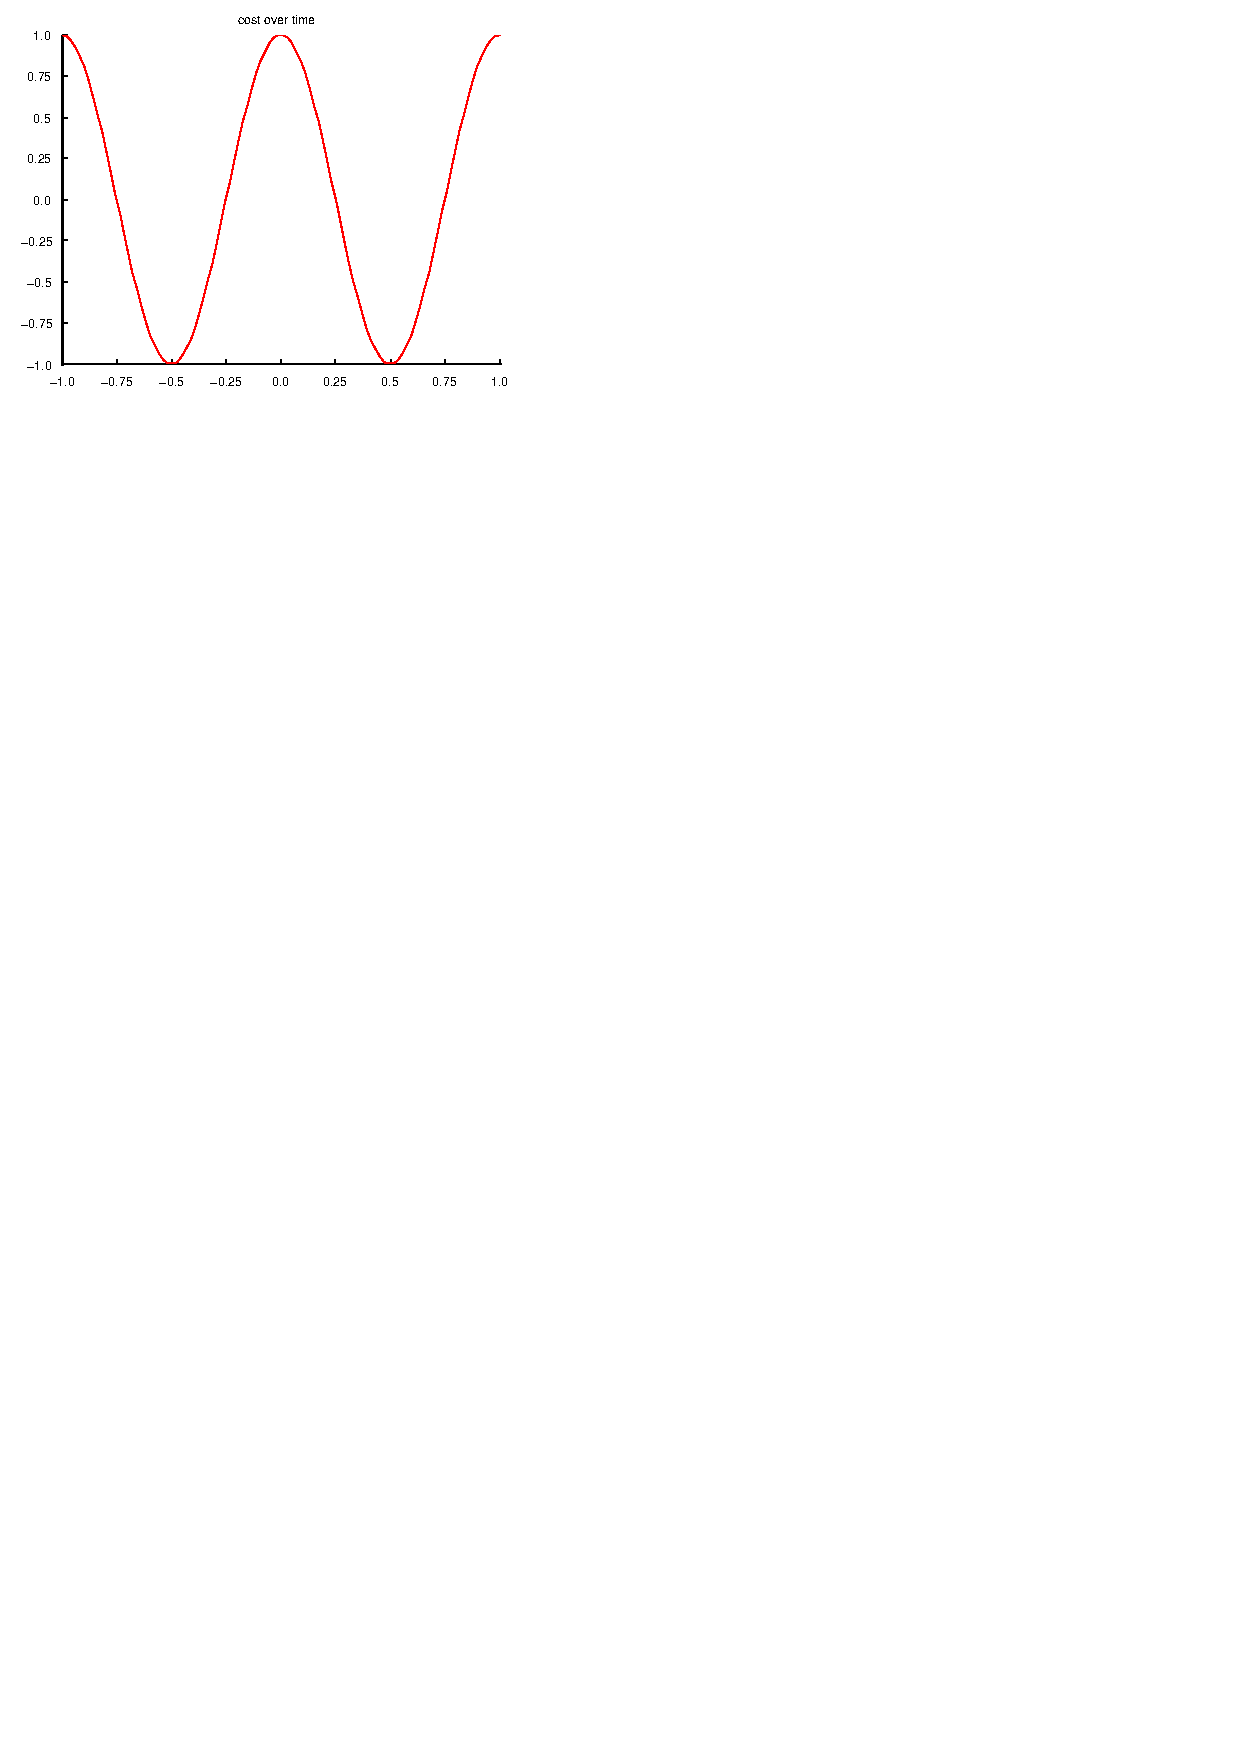
\includegraphics[width=8cm]{title1}}

We now increase the size of the font using the properties
of the \verb|label|
\begin{verbatim}
--> title('cost over time','fontsize',20);
Warning: Newly defined variable nargin shadows a function of the same name.  Use clear nargin to recover access to the function
\end{verbatim}


\centerline{\includegraphics[width=8cm]{title2}}

